\documentclass[a4paper,12pt,oneside]{scrbook}
\usepackage{amsmath,amssymb,amsthm,mathrsfs}
\usepackage{datetime}
\usepackage{hyperref}
\usepackage{graphicx}
\usepackage[ngerman]{babel}
\usepackage{bigfoot} %% Für grosse Fussnoten
\usepackage{makeidx}

\newtheorem*{crucial}{Crucial Observation}
\newtheorem*{warning}{Warning}


\def\AA{\mathbb{A}}
\def\BB{\mathbb{B}}
\def\EE{\mathbb{E}}
\def\HH{\mathbb{H}}
\def\DD{\mathbb{D}}
\def\NN{\mathbb{N}}
\def\RR{\mathbb{R}}
\def\TT{\mathbb{T}}
\def\CC{\mathbb{C}}
\def\ZZ{\mathbb{Z}}
\def\PP{\mathbb{P}}
\def\QQ{\mathbb{Q}}
\def\FF{\mathbb{F}}
\def\GG{\mathbb{G}}
\def\LL{\mathbb{L}}
\def\MM{\mathbb{M}}
\def\SS{\mathbb{S}}
\def\UU{\mathbb{U}}
\def\XX{\mathbb{X}}


%%% Philipp's macros

\newcommand{\dom}[1]{{\mathrm {dom}}({#1})}
\newcommand{\sman}[1]{{#1}^{\mathrm{sm,an}}}
\newcommand{\ansm}[1]{{#1}^{\mathrm{an,sm}}}
\newcommand{\sm}[1]{{#1}^{\mathrm{sm}}}
\newcommand{\anE}{\mathrm{an}}
\newcommand{\an}[1]{{#1}^{\anE}}
\newcommand{\stab}[1]{{\mathrm{Stab}(#1)}}


\newcommand{\hgtexp}{S}

\newcommand{\rank}{{\mathrm{rank}}\,}
\newcommand{\atopx}[2]{{\genfrac{}{}{0pt}{}{#1}{#2}}}
\newcommand{\IP}{{\PP}}
\newcommand{\IF}{{\FF}}
\newcommand{\IG}{{\GG}}
\newcommand{\IH}{{\HH}}
\newcommand{\IC}{{\CC}}
\newcommand{\IR}{{\RR}}
\newcommand{\IT}{{\TT}}
\newcommand{\IRan}{{{\RR}_{\mathrm{an}}}}
\newcommand{\IRexp}{{{\RR}_{\mathrm{exp}}}}
\newcommand{\IRanexp}{{{\RR}_{\mathrm{an,exp}}}}
\newcommand{\RRan}{{\IRan}}
\newcommand{\RRanexp}{{\IRanexp}}
\newcommand{\IRalg}{{\RR}_{\mathrm{alg}}}
\newcommand{\IQbar}{{\overline{\QQ}}}
\newcommand{\Kbar}{{\overline{K}}}
\newcommand{\IZ}{{\ZZ}}
\newcommand{\IN}{{\NN}}
\newcommand{\IA}{{\AA}}
\newcommand{\IQ}{{\QQ}}
\newcommand{\IQpbar}{{\overline{\QQ}_p}}
\newcommand{\IQp}{{\QQ_p}}
\newcommand{\ts}[1]{{T}_0({#1})}

\newcommand{\cS}{{\mathcal S}}
\newcommand{\cA}{{\mathcal A}}
\newcommand{\cB}{{\mathcal B}}
\newcommand{\cC}{{\mathcal C}}
\newcommand{\cE}{{\mathcal E}}
\newcommand{\cF}{{\mathcal F}}
\newcommand{\cK}{{\mathcal K}}
\newcommand{\cL}{{\mathcal L}}
\newcommand{\cM}{{\mathcal M}}
\newcommand{\cO}{{\mathcal O}}
\newcommand{\cV}{{\mathcal V}}
\newcommand{\cW}{{\mathcal W}}
\newcommand{\cX}{{\mathcal{X}}}
\newcommand{\cY}{{\mathcal Y}}
\newcommand{\cZ}{{\mathcal Z}}



\newcommand{\defZ}{Z}
\newcommand{\defF}{F}
\newcommand{\defW}{W}
\newcommand{\defC}{C}
\newcommand{\defE}{E}
%\newcommand{\deffam}{F}



\newcommand{\mat}[2]{\mathrm{Mat}_{#1}({#2})}
\newcommand{\ssm}{\smallsetminus}
\newcommand{\ord}[1]{{\rm ord}({#1})}
\newcommand{\opt}[2]{{\rm Opt}_{#2}({#1})}
\newcommand{\Height}[1]{{H}({#1})}
\newcommand{\trdeg}{{\rm trdeg\,}} 
\newcommand{\geo}[1]{\langle {#1}\rangle_{{\rm geo}}}
\newcommand{\defect}{\delta}
\newcommand{\geodef}{{\delta_{\rm geo}}}
\newcommand{\en}[1]{{\rm End}({#1})}
\newcommand{\Hom}[1]{{\rm Hom}({#1})}
\newcommand{\hommaxR}[1]{\text{\rm Hom}({#1})^{*}_{\IR}}
\newcommand{\arith}{\rm arith}
\newcommand{\sgu}[2]{{#1}^{[{#2}]}}
\newcommand{\oa}[1]{{#1}^{\rm oa}}
\newcommand{\codim}{{\rm codim}}
\newcommand{\lgo}{LGO}
\newcommand{\zcl}[1]{{\rm Zcl}({#1})}


\newcommand{\trans}[1]{{#1}^{T}}

\newcommand{\red}[1]{\textcolor{red}{#1}}

\renewcommand{\subset}{\subseteq} %%% Some people think \subset
%%% excludes equality
\renewcommand{\supset}{\supseteq}

\newcommand{\gra}[1]{\mathrm{Gr}({#1})}


\newcommand{\gl}[2]{{\mathrm {GL}}_{#1}({#2})}
\renewcommand{\sp}[2]{{\mathrm {Sp}}_{#1}({#2})}
\newcommand{\autS}{{\mathrm {Aut}}}
\newcommand{\aut}[1]{\autS({#1})}

\newcommand{\spec}[1]{\mathrm{Spec}\,{#1}}

\newcommand{\tor}[1]{{#1}_{\mathrm{tor}}}
\newcommand{\gal}[1]{{\mathrm{Gal}}({#1})}


\newcommand{\zeroset}[1]{\mathscr{Z}({#1})}


\newcommand{\jac}{\mathrm{Jac}}

\newcommand{\bfzeta}{{\boldsymbol{\zeta}}}

\newcommand{\mattt}[4]
{\left(
  \begin{array}{cc}
    {#1} & {#2} \\ {#3} & {#4} 
  \end{array}
\right)}

\newcommand{\matto}[2]
{\left(
  \begin{array}{c}
    {#1} \\ {#2}
  \end{array}
\right)}

\newcommand{\matot}[2]
{\left(
  \begin{array}{cc}
    {#1} & {#2}
  \end{array}
\right)}

\newcommand{\be}{\mathbf{e}}

\let\emph\textbf

\newcommand{\absgalk}{\mathrm{Gal}(\overline{K}/K)}
\makeindex

\begin{document}

\title{Elliptische Kurven und ihre Anwendung in der Kryptographie}
\subtitle{DMK-Weiterbildung vom 8. September 2022}
\author{Philipp~Habegger \\ Departement Mathematik und Informatik
 \\ Universität Basel \\ \texttt{philipp.habegger@unibas.ch}}
\date{\small{Revision vom \today{} um
    \currenttime}}%\\\texttt{\input{{.git/refs/heads/master}}}}


\maketitle
\tableofcontents

\setcounter{chapter}{-1}

\chapter{Vorwort}

Der Inhalt dieses Skripts bildet die Grundlage der
Weiterbildungsveranstaltung der Deutschschweizerische
Mathematik-Kommission vom 8. September 2022, welche ich an der
Universität Basel gehalten habe.

Ich bin dankbar um die Meldung von Fehlern und Ungenaugigkeiten an
meine Email-Adresse auf der Titelseite.

\section{Notation}

Wir verwenden die folgenden Konventionen.

\begin{itemize}
\item Die Menge der natürlichen Zahlen ist $\IN = \{1,2,3,\ldots\}$.

\item Wir wählen eine Nullstelle von $X^2+1$ in $\IC$ und bezeichnen sie
  mit $\sqrt{-1}$.
  
\end{itemize}

%%% Local Variables:
%%% TeX-master: "main"
%%% End:


\chapter{Kongruente Zahlen}

\begin{definition}
  Eine natürliche Zahl $n\in\IN$ heisst \emph{kongruente
    Zahl}\index{Kongruente Zahl}, falls
  $n$ die Fläche eines rechwinkligen Dreiecks mit rationalen
  Seitenlängen ist. 
\end{definition}

\begin{bemerkung}
  Per Definition ist $n$ genau dann eine kongruente Zahl, wenn es positive
  $a,b,c\in\IQ$ gibt, so dass $a^2+b^2=c^2$ und $n = ab/2$. 
\end{bemerkung}

\begin{beispiel}\leavevmode
  \begin{enumerate}
  \item [(i)]
    Die Zahl $n=6$ ist kongruent, da es ein rechtwinkliges Dreieck mit Seitenlängen
    $a=3,b=4,c=5$  gibt und da $6=3\cdot 4/2$. 
  \item[(ii)]
    Für jede kongruente Zahl $n$ und jede rationale Zahl
    $\lambda\not=0$ ist $\lambda^2 n$ eine kongruente Zahl, sofern es
    eine ganze Zahl ist. Um das zu
    beweisen, dürfen wir $\lambda > 0$ annehmen. Nach Voraussetzung
    ist $n=ab/2$ mit $a^2+b^2=c^2$. Also ${a'}^2+{b'}^2={c'}^2$, wobei
    $a'=\lambda a, b'=\lambda b, c'=\lambda c$ wiederum rational.
    Die Fläche des entsprechenden rechtwinkligen Dreiecks ist die
    Zahl $a'b'/2
    = \lambda^2 ab/2 = \lambda^2 n$ kongruent, falls sie ganz ist.
  \item[(iii)]
    Aus (i) und (ii) folgt, dass es unendlich viele kongruente Zahlen
    gibt, denn $\{6\lambda^2 : \lambda\in\IN\}$ besteht aus kongruente
    Zahlen.
    Weiterhin ist jede kongruente Zahl ein rationales Vielfaches
    einer quadratfreien kongruenten Zahl.

  \item[(iv)] Es gilt $(3/2)^2 +(20/3)^2 = (41/6)^2$  und damit ist
    $n=5= (3/2)\cdot(20/3)/2$ kongruent.
    
  \item[(v)] Auch $n=7$ ist kongruent wegen $(35/12)^2 +
    (24/5)^2=(337/60)^2$.

  \end{enumerate}  
\end{beispiel}
Für jedes Tripel $(a,b,c)$ mit $a,b,c$ positive rationalen Zahlen mit
$a^2+b^2=c^2$ existieren $u>v>0$ rational mit $a =
u^2-v^2,b=2uv,c=u^2+v^2$. Hieraus können wir auf systematische Art
alle kongruente Zahlen produzieren. Es gilt folgt folgende Aussage.

\begin{lemma}
  Die Menge der kongruenten Zahlen ist
  $$
  \{ n \in \IN : \text{ es gibt $u>v>0$ in $\IQ$ mit $n=(u^2-v^2)uv$ }
  \}.
  $$
\end{lemma}


Ist $n=1$ eine kongruente Zahl? Die Antwort ist nein und dies wurde
von Pierre Fermat bewiesen.

\begin{satz}[Fermat]
  Eins  ist keine kongruente Zahl.
\end{satz}
\begin{proof}
  TODO
\end{proof}

\begin{korollar}
  Die reelle Zahl $\sqrt{2}$ ist irrational. 
\end{korollar}
\begin{proof}
  Es gilt $a^2+b^2=2^2$ und $ab/2=1$ für $a=b=\sqrt 2$. Aber $1$ ist
  nicht eine kongruente Zahl wegen Fermats Satz. Damit kann $\sqrt 2$
  nicht rational sein.
\end{proof}

Eine klassische Fragestellung ist das folgende Problem.

\begin{problem}
  Gegeben eine natürliche Zahl $n$. Ist $n$ eine kongruente Zahl oder
  nicht? 
\end{problem}

Es ist heute kein Algorithmus bekannt, der entscheidet, ob eine
gegebene natürliche Zahl kongruent ist oder nicht. Daher kennen wir
keinen systematischen Zugang zu der Frage oben.

In der Definition von kongruente Zahl kommen 

\begin{lemma} \label{lem:congruentelliptic}
  Sei $n\in\IN$. 
  \begin{enumerate}
  \item
  Seien $a,b,c\in \IQ$ mit $a^2+b^2=c^2,a\not=c$ und $n = ab/2$. Wir definieren
  \begin{equation*}
    x = \frac{nb}{c-a} \quad\text{und}\quad
    y = \frac{2n^2}{c-a}. 
  \end{equation*}
  Dann gilt $y^2 = x^3-n^2 x$.
  \item Seien $x,y\in\IQ$ mit $y^2 = x^3-n^2x$. Falls $y\not=0$, dann
    ist $n$ eine kongruente Zahl.
  \end{enumerate}
\end{lemma}
\begin{proof}
  Teil (i) ist eine direkt Rechnung. Es gilt
  \begin{equation*}
    y^2 = \frac{4n^4}{(c-a)^2} = \frac{a^4b^4}{4(c-a)^2} 
  \end{equation*}
  und
  \begin{alignat*}1
    x^3 -n^2 x &= n^3 \frac{b^3}{(c-a)^3} - n^3 \frac{b}{c-a}
    = n^3 \frac{b}{c-a}\left(\frac{b^2}{(c-a)^2}-1\right)
    = n^3 b\frac{b^2-(c-a)^2}{(c-a)^3}
    = \frac{a^3b^4}{8}\frac{b^2-(c-a)^2}{(c-a)^3}.
  \end{alignat*}
  Es gilt  $$
  y^2 - (x^3-n^2x) = \frac{a^3b^4}{8(c-a)^3} \left(
    2a(c-a) - b^2+(c-a)^2\right) =
  \frac{a^3b^4}{8(c-a)^3} (c^2-a^2-b^2)=0,
  $$
  was für (i)  zu zeigen.

  Für den Beweis von (ii) setzen wir
  \begin{equation*}
    a = \left|\frac{n^2-x^2}{y}\right|, \quad
    b = \left|\frac{2nx}{y}\right|, \quad\text{und}\quad
    c = \left|\frac{n^2+x^2}{y}\right|. 
  \end{equation*}
  Eine direkt Rechnung zeigt $a^2+b^2=c^2$. Weiterhin gilt
  \begin{equation*}
    \frac{ab}{2} = \frac{|(n^2-x^2)(2nx)|}{2y^2} = \frac{2n |n^2x -
      x^3|}{2y^2} = \frac{n |-y^2|}{y^2} = n.
  \end{equation*}

  Da $a,b,c$ nicht negative rationale Zahlen sind, reicht es zu
  zeigen, dass $abc\not=0$. Es gilt $c = (n^2+x^2)/|y| \ge n^2/|y|>0$.

  Es gilt $y^2 = (x^2-n^2)x\not=0$. Daraus folgt 
  $x^2-n^2\not=0$ und $x\not=0$. Also folgt $a\not=0$ und $b\not=0$. 

  Es folgt, dass $n$ eine kongruente Zahl ist. 
\end{proof}

Für jede natürliche Zahl $n\in\IN$ definiert
Lösungsmenge der kubischen Gleichung
\begin{equation}
  \label{eq:ellipticcong}
  Y^2 = X^3-n^2X  
\end{equation}
definiert eine Kurve in der reelle (oder komplexen) Ebene. Von besonderem Interesse sind die
rationalen Punkte dieser Kurve, d.h. Punkte, deren Koordinaten
rational sind.

Die Punkte $(0,0),(\pm n,0)$ liegen augenscheinlich auf der Kurve für
jedes $n$. Gibt es mindestens ein weiterer rationaler Punkt, d.h. ein
Punkt dessen Ordinate nicht verschwindet, so ist $n$ eine kongruente
Zahl.
Weiterhin ist die Umkehrung auch wahr. 


Die Gleichung (\ref{eq:ellipticcong}) ist ein Spezialfall der
Weierstrass-Gleichung, welche im Allgemeinen eine elliptische Kurve
definiert. 
%%% Local Variables:
%%% TeX-master: "main"
%%% End:



\chapter{Elliptische Kurven}

In diesem Abschnitt werden elliptische Kurven ad hoc eingeführt.
Teil des Datums einer elliptischen Kurve ist ein Grundkörper $K$. Dies
ist a priori ein beliebiger Körper. Aber für uns sind die wichtigsten
Wahlen von Grundkörper die rationalen Zahlen $\IQ$, die reellen Zahlen
$\IR$ und die komplexen Zahlen $\IC$. Für Anwendungen in der
Krytographie spielen  die endlichen Körper eine zentrale Rolle.


Es sei angemerkt, dass die Theorie elliptische Kurven im
arithmetischen Fall, d.h. für den  $K=\IQ$ und verwandte Körper, ihre
volle Tiefe entfaltet. Falls der Grundkörper, so wie $\IC$,
algebraisch abgeschlossen ist, verschwinden die arithmetischen
Aspekte.


\section{Definition der Elliptischen Kurve}

\begin{definition}
  Sei $K$ wie oben ein Körper.
  Eine \emph{Weierstrass-Gleichung}\index{Weierstrass-Gleichung} ist eine Gleichung vom Typ
  \begin{equation}
    \label{eq:weierstrass}
    E: Y^2 = X^3 + aX+b
  \end{equation}
  mit Unbekannten $X,Y$ und Koeffizienten $a,b\in K$, welche die
  Bedingung
  \begin{equation}
    \label{eq:disccondition}
    \Delta_E = -2^4(4a^3+27b^2)\not=0
  \end{equation}
  erfüllt. Die Grösse $\Delta_E$, ein Element aus $K$, heisst
  \emph{Diskriminante}\index{Diskriminante einer Weierstrass-Gleichung}
  der Weierstrass-Gleichung $E$. Zur Weierstrass-Gleichung $E$ gehört
  das Weierstrass-Polynom\footnote{Diese Beizeichnung ist nicht
    standard.} $Y^2- (X^3+aX+b)$.
\end{definition}

\begin{beispiele}\leavevmode
  \begin{enumerate}
  \item [(i)] In (\ref{eq:ellipticcong}) hatten wir die Gleichung $Y^2 = X^3-n^2X$
    für $n\in\IN$ betrachtet. Es handelt sich um eine
    Weierstrass-Gleichung $E_n$, für $K=\IQ$ (oder jeden Körper, der $\IQ$
    enthält) mit $\Delta_{E_n} = -2^4 3^3 n^4$.
  \item[(ii)] Die Gleichung
    \begin{equation*}
      Y^2 = X^3,
    \end{equation*}
    definiert keine Weierstass-Gleichung, da (\ref{eq:disccondition})
    nicht erfüllt ist.
  \end{enumerate}
\end{beispiele}

\begin{bemerkung}
  Sei $K$ ein Körper der Charakteristik $2$, z.B. $K=\IF_2$, und
  $a,b\in K$. Dann ist $Y^2 = X^3+aX+b$ keine Weierstrass-Gleichung,
  da (\ref{eq:disccondition}) nicht erfüllt ist. In $K$ gilt $2=0$.

  Das ist  unbefriedigend, da für Anwendung in der Kryptographe
  endliche Körper 
  der Charakteristik $2$ wichtig sind. Um Charakteristik $2$ (und auch
  $3$) abzudecken, muss man die Definition von Weierstrass-Gleichung
  verallgemeinern. Wir werden dies hier nicht tun, da es etwas
  technisch ist. Kurzum reicht es mit den sogenannten langen
  Weierstrass-Gleichungen vom Typ
  \begin{equation*}
    Y^2 + a_1 XY + a_3 Y = X^3+a_2 X^2 + a_4 X + a_6
  \end{equation*}
  mit entsprechender (aber kompliziertere) Diskriminanten-Bedingung
  \begin{alignat*}1
    &-a_6 a_1^6 + a_4 a_3 a_1^5 + ((-a_3^2 - 12 a_6) a_2 + a_4^2) a_1^4 +
    (8 a_4 a_3 a_2 + (a_3^3 + 36 a_6 a_3)) a_1^3\\
    &+ ((-8 a_3^2 - 48 a_6) a_2^2 +
    8 a_4^2 a_2 +
    (-30 a_4 a_3^2 + 72 a_6 a_4)) a_1^2 \\
    &+ (16 a_4 a_3 a_2^2 +
    (36 a_3^3 + 144 a_6 a_3) a_2 - 96 a_4^2 a_3) a_1 \\
    &+ ((-16 a_3^2 -
    64 a_6) a_2^3 + 16 a_4^2 a_2^2 + (72 a_4 a_3^2 + 288 a_6 a_4) a_2
    \\
    & +
    (-27 a_3^4 - 216 a_6 a_3^2 + (-64 a_4^3 - 432 a_6^2))) \not=0.
  \end{alignat*}
  zu arbeiten.

  In Charakteristik $\not=2$ und $\not=3$ kann man jede lange
  Weierstrass-Gleichung mittels quadratisch und kubischem Ergänzen
  durch eine affine lineare Transformation auf eine
  Weierstrass-Gleichung umformen. 
\end{bemerkung}

Nun wollen wir die Bedingung (\ref{eq:disccondition}) rechtfertigen.
Die partiell Ableitung eines Polynoms ist formal über jedem Körper
definiert, es ist kein Grenzwertbegriff notwendig.

\begin{lemma}
  \label{lem:smooth}
  Sei $F$ das Weierstrass-Polynom einer Weierstrass-Gleichung
  (\ref{eq:weierstrass}). Sei $(x,y)\in K^2$ mit $F(x,y)\not=0$. Dann
  gilt
  \begin{equation*}
    \frac{\partial F}{\partial X}(x,y)\not=0 \qoq
    \frac{\partial F}{\partial Y}(x,y)\not=0.
  \end{equation*}
\end{lemma}
\begin{proof}
  Es gilt $F = Y^2 - X^3-aX-b$ und $-2^4(4a^3+27b^2)\not=0$.
  Insbesondere gilt $2\not=0$ in $K$. Weiterhin
  \begin{equation*}
    \frac{\partial F}{\partial Y} = 2Y. 
  \end{equation*}

  Sicher ist diese Ableitung $\not=0$ an jedem Punkt $(x,y)$ mit
  $y\not=0$.
  Es reicht also zu zeigen, dass $    \frac{\partial F}{\partial
    X}(x,0)\not=0$, falls $F(x,0)=0$.

  Nun gilt
  \begin{equation*}
    \underbrace{(X^3+aX+b)}_{=F}(288aX-432b) +
    \underbrace{(-3X^2-a)}_{= \partial F/\partial X}(96aX^2 - 144bX + 64a^2)
    = -2^4(4a^3+27b^2) \not=0
  \end{equation*}
  nach Voraussetzung.
  Wir substituieren $X$ durch $x$ und finden 
  $\frac{\partial F}{\partial
    X}(x,0)\not=0$ da $F(x,0)$.  
\end{proof}

\begin{bemerkung}
  \label{bem:tangente}
  Im Fall $K=\IR$ können wir dieses letzte Lemma geometrisch wie folgt
  interpretieren.
  Sei $(x,y)\in\IR^2$ eine Nullstelle von $F$, dem Weierstrass-Polynom
  einer Weierstrass-Gleichung. Wir setzen
  $$\alpha = -\frac{\partial F}{\partial Y}(x,y) \quq
  \beta = \frac{\partial F}{\partial X}(x,y).$$
  Dann ist $(\alpha,\beta)$ nicht der Nullvektor.

  Aus dem Satz von der impliziten Funktion folgt, wir die
  Nullstellenmenge von $F$ in $\IR^2$ in der Nähe von $(x,y)$ durch
  den Graph einer glatten Funktion (nach einem möglichen Koordinatentausch)
  ausdrücken können. 

  Weiterhin ist die Menge
  \begin{equation*}
    T = \{(x+\alpha t,y+\beta t) : t\in\IR\}
  \end{equation*}
  eine Gerade durch $(x,y)$. Wir definieren $f(t) =
  F(x+t\alpha,y+t\beta)$ für alle $t\in\IR$. 
  Dann gilt 
  \begin{equation*}
    \frac{d\gamma}{dt}(t)
    = \underbrace{F(x,y)}_{=0} + \left(\underbrace{\alpha \frac{\partial F}{\partial X}(x,y)
    +\beta \frac{\partial F}{\partial Y}(x,y)}_{=0}\right)t + \text{(Terme der
      Ordnung $\ge 2$ in $t$)}.
  \end{equation*}
  
  Also hat $t\mapsto F(x+t\alpha,y+t\beta)$ eine mehrfache Nullstelle
  bei $t=0$. Dies bedeutet, dass $T$ die Tangent an der
  Nullstellenmenge von $F$ ist.

  Zusammengefasst: die Gerade durch $(x,y)$ mit Richtungsvektor
  \begin{equation*}
    \left(-\frac{\partial F}{\partial Y}(x,y),\frac{\partial F}{\partial X}(x,y)\right)
  \end{equation*}
  liegt tangential an der Nullstellenmenge von $F$.
\end{bemerkung}

Die Schlussfolgerung von Lemma~\ref{lem:smooth} besagt, dass die
Nullstellenmenge einer Weierstrass-Gleichung an jedem Punkt einer
Bedingung genügt, welche sich zumindest im reellen Fall
als ``Glattheitsbedigung'' verstehen lässt.

\begin{definition}
  \label{def:tangentensteigung}
  Sei $F$ das Weierstrass-Polynom einer Weierstrass-Gleichung. Falls
  $(x,y)\in K$ und $y\not=0$, dann heisst
  \begin{equation*}
    \frac{\frac{\partial F}{\partial X}}{-\frac{\partial F}{\partial
        Y}}(x,y) = \frac{3x^2+a}{2y}
  \end{equation*}
  \emph{Tangentensteigung} an $(x,y)$. 
\end{definition}

Sei $m$ die Tangentensteigung an $(x,y)$.
So wie in Beispiel \ref{bem:tangente} zeigt man, dass
$F(x+t,y+mt)$ bei $t=0$ eine Nullstelle der Ordnung $\ge 2$ hat. 

\begin{beispiel}
  Die Lösungsmenge von $Y^2=X^3$ hat bei $(0,0)$ eine ``Spitze''.  Die
  Nullstellenmenge ist an diesem Punkt nicht glatt, vgl.
  Abbildung~\ref{fig:cusp} links.

  \begin{figure}
    \centering    
    \caption{Lösungsmenge von $Y^2=X^3$ (links) und $Y^2 = X^3-X$ (rechts)}
    \label{fig:cusp}
    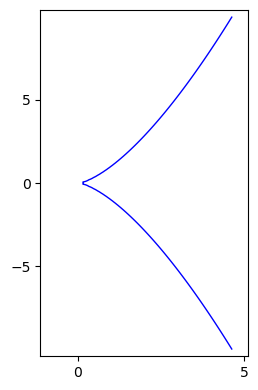
\includegraphics[width=0.3\textwidth]{./plots/cusp.png}
    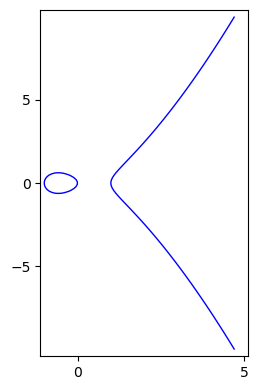
\includegraphics[width=0.3\textwidth]{./plots/smooth_n_equal_1.png}
  \end{figure}

  In der gleichen Abbildung rechts ist eine glatte Kurve zu sehen.
\end{beispiel}

\section{Das Gruppengesetz}

In diesem Abschnitt werden wir zeigen, wie man auf der Lösungsmenge
einer Weierstrass-Gleichung zusammen mit einem zusätzlichen Punkt,
eine Gruppenstruktur definieren kann. Die Konstruktion kann man rein
geometrisch veraschaulichen. Wie oben bezeichnet $K$ ein Körper in dem
sich alles abspielt (sofern nicht anders vermerkt). 

\begin{definition}
  Sei $Y^2 = X^3+aX+b$ eine Weierstrass-Gleichung $E$.
  Wir definieren 
  \begin{equation*}
    E(K) = \{(x,y) \in K^2 : y^2 = x^3 + ax+b\} \cup \{\cO\}.
  \end{equation*}
  wobei $\cO$ zunächst ein weiteres Element ist, welches nicht in
  $K^2$ liegt. Man nennt $E(K)$ die \emph{Menge der $K$-rationalen Punkten
  von $E$}. 
\end{definition}

\begin{beispiel}
  \label{bsp:fermat}
  Für die Weierstrass-Gleichung $E$ gegeben durch $Y^2 = X^3-X$ und
  für $K=\IQ$ besagt der 
  Satz von Fermat, Satz~\ref{satz:fermat2}, dass
  $$ E(\IQ) = \{(0,0), (\pm 1,0), \cO\} .$$
  aus vier Elementen besteht. 
\end{beispiel}

Wir werden zeigen, dass wir $E(K)$ mit der Struktur einer abelschen
Gruppe verstehen können.
Dazu müssen wir eine Verknüpfung $+\colon E(K)\times
E(K)\rightarrow E(K)$, eine Inversionsabbildung
$-\colon E(K)\rightarrow E(K)$, sowie ein neutrales Element in $E(K)$
produzieren.



\subsection{Die Verknüpfung}
\label{sec:verknuepfung}

Sei $E$ eine Weierstrass-Gleichung gegeben durch $Y^2 = X^3+aX+b$ mit
$a,b\in K$. 
In einem ersten Schritt werden wir eine Verknüpfung
\begin{equation*}
  + \colon E(K)\times E(K) \rightarrow E(K)
\end{equation*}
definieren. Es ist üblich, die Verknüpfung mit ``$+$'' zu bezeichnen.
Später werden wir feststellen, dass die so konstruierte Gruppe eine
abelsche Gruppe ist. 

Seien $P$ und $Q$ Elemente von $E(K)$. Es folgt eine Aufspaltung in
verschiendene Fälle. Wir werden bereits in der Konstruktion
überprüfen, dass die Verküpfung $+$ die Bedingung
$$
P+Q=Q+P\quad\text{für alle}\quad P,Q\in E(K) 
$$
erfüllt. Hieraus werden wir folgern, dass die Gruppe $E(K)$ abelsch
ist.  

\medskip
\textbf{Fall 1: Die Menge $\{P,Q,\cO\}$ hat drei Elemente.} In diesem
Fall gilt $P = (x_1,y_1)$ und $Q = (x_2,y_2)$. Weiterhin haben wir
$P\not=Q$.
Daher gibt es genau eine Gerade $G$ durch $P$ und $Q$.

Wir unterscheiden zwei Unterfälle. 

\textbf{Unterfall 1a. Es gilt $x_1\not=x_2$.} In diesem Fall hat die
Gerade $G$ (endliche) Steigung $m = \frac{y_2-y_1}{x_2-x_1}\in K$. In
anderen Worten, sie hat die Gesalt
\begin{equation*}
  G = \{(x,mx+q) : x\in K \}
\end{equation*}
mit $q=y_1-m x_1$. Vgl. Abbildung \ref{fig:unterfall1a} darin ist $G$
gestrichelt.

\begin{figure}
  \centering    
  \caption{$E: Y^2 = X^3-5^2 X,P = (-4,6),Q = (\frac{1681}{144},-\frac{62279}{1728})$}
  \label{fig:unterfall1a}
  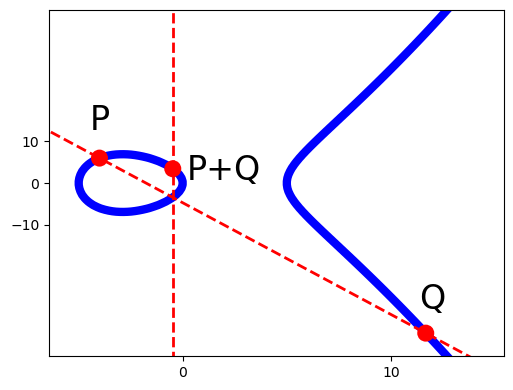
\includegraphics[width=0.3\textwidth]{./plots/unterfall1a.png}
\end{figure}
 
Daher sind $P$ und $Q$ Schnittpunkte der Gerade $G$ mit der Menge
$E(K)\ssm \{\cO\}$. Mit Vielfachheiten gezählt hat die Gerade $G$
jedoch drei Schnittpunkte mit der Lösungsmenge von $Y^2=X^3+aX+b$. Wir
können dies wie folgt direkt überprüfen. Dazu defineren wir
das Polynom
\begin{equation*}
  A = (mX+q)^2 - (X^3+aX+b) =-X^3+m^2X +\text{(Terme von Grad $\le 1$ in $X$)}
  \in K[X]. 
\end{equation*}

Das Polynom $A$ hat Grad $3$  und wir kennen bereits zwei verschiedene
Nullstellen: $x_1,x_2\in K$. Daher lässt sich $A$ durch $X-x_1$ und
$X-x_2$ teilen. Es gilt also $A = -(X-x_1)(X-x_2)(X-x_3)$, dabei muss
$x_3$ als wiederum ein Element in $K$ sein, denn es gilt $x_1+x_2+x_3
= m^2$, also
\begin{equation*}
  x_3 = \left(\frac{y_2-y_1}{x_2-x_1}\right)^2-x_2-x_1.
\end{equation*}
Nach Konstruktion ist das Paar $(x_3,y_3)$ mit  $y_3=mx_3+q$ eine
Nullstelle von $Y^2-(X^3+aX+b)$. Weiterhin ist auch $(x_3,-y_3)$ eine
Nullstelle.

In Unterfall 1a definieren wir
\begin{equation*}
  P+Q = (x_3,-y_3) \in E(K)\ssm \{\cO\}.
\end{equation*}

Sind wir in  Unterfall 1a, so ist auch das Paar $(Q,P)$ in Unterfall
1a. Es gilt $P+Q=Q+P$, da die Gerade und sowohl $(m,q)$ unabhängig von
der Reihenfolge von $P,Q$ ist. 

\textbf{Unterfall 1b. Es gilt $x_1=x_2$.} Nun liegt die Gerade $G$
senkrecht zur Abszisse, vgl. Abbildung~\ref{fig:unterfall1b}. Es gilt
\begin{equation*}
  y_1^2 = x_1^3+a x_1 +b = x_2^3+a x_2 +b = y_2^2
\end{equation*}
und daher $y_1=-y_2$ da $P\not=Q$. Nun stehen wir vor einem
Dilemma, die Gerade $G$ hat keine weiteren Schnittpunkte mit $E(K)$ in
der Ebene $K^2$. Jetzt kommt uns der Punkt $\cO$ zur Hilfe.

In Unterfall 1b definieren wir
\begin{equation*}
  P+Q = \cO \in E(K).
\end{equation*}

Vertauscht man $P,Q$ so bleiben wir in Unterfall 1b und es gilt
trivialerweise $P+Q=Q+P$.  

\begin{figure}
  \centering    
  \caption{$E: Y^2 = X^3-5^2 X,P = (-4,6),Q = (-4,-6)$}
  \label{fig:unterfall1b}
  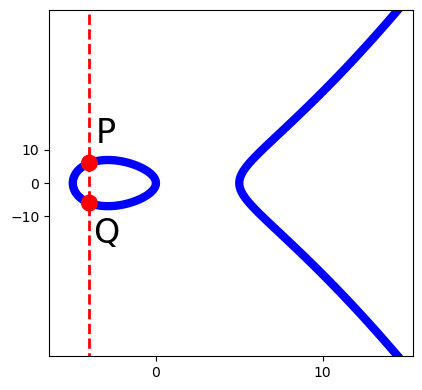
\includegraphics[width=0.3\textwidth]{./plots/unterfall1b.png}
\end{figure}

\medskip
\textbf{Fall 2: Die Menge $\{P,Q,\cO\}$ hat zwei Elemente.} Auch hier
gibt es mehrere Unterfälle.

\textbf{Unterfall 2a: Es gilt $P=Q\not=\cO$ und $P=(x,y)$ mit $y\not=0$.}
%Wir schreiben $P=Q=(x,y)$ mit $x,y\in K$.

Die Gerade, welche in Fall 1 konstruiert wurde, ist nun nicht
eindeutig bestimmt.

Etwas Intuition schafft die folgende Überlegung. Wir
versetzen uns in die reelle Welt und ersetzen den Punkte $Q$ durch
eine Folge von Punkten $(Q_n)_{n\in\IN}$ aus $E(\IR)\ssm\{Q,\cO\}$, dessen
Koordinaten für $n\rightarrow\infty$ gegen $Q=P$ konvergieren.
Die Gerade $G_n$ durch $P$ und $Q_n$ ist wohldefiniert und die Summe
$P+Q_n$ lässt sich mit der Vorschrift aus Fall 1 bestimmen.
Anschaulich nähert sich die Gerade $G_n$ der Tangente and
$E(\IR)\ssm\{\cO\}$ durch den Punkte $P$. Vgl.
Abbildung~\ref{fig:unterfall2a}. 

\begin{figure}
  \centering    
  \caption{$E: Y^2 = X^3-5^2 X,P = Q=(-4,6)$}
  \label{fig:unterfall2a}
  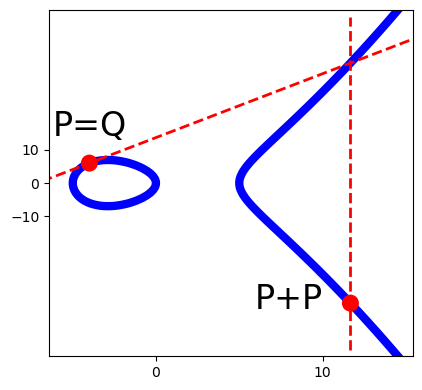
\includegraphics[width=0.3\textwidth]{./plots/unterfall2a.png}
\end{figure}

Für einen allgemeinen Körper können wir zwar nicht mit solchen
Grenzbegriffen argumentieren, aber wir haben einen Ersatz für die
Tangente in Bemerkung~\ref{bem:tangente} und Definition
\ref{def:tangentensteigung}
gefunden.


Für $y\not=0$ dürfen wir  Definition \ref{def:tangentensteigung}
anwenden. Das weitere Vorgehen ist vergleichbar mit Unterfall 1a.
Wir setzen
$$m =  \frac{3x^2+a}{2y}\in K\quq q = y-mx\in K.$$
Das Polynom
$$
A = (mX+a)^2 - (X^3+aX+b) \in K[X]
$$
hat nur eine Nullstelle der Ordnung $\ge 2$ in $x$. Dies lässt sich
rein formal mit Hilfe der Definition von $m$ überprüfen.
Also gilt $A = -(X-x)^2(X-x')$ für ein $x'\in K$. Dabei gilt
\begin{equation*}
  x' = m^2 - 2x = \left(\frac{3x^2+a}{2y}\right)^2 - 2x. 
\end{equation*}

Der Punkt $(x',y')$ mit $y'=mx'+q$ liegt in $E(K)$. Wie in Unterfall
1a liegt $(x',-y')$ auch in $E(K)$. 
In Unterfall 2a
definieren wir
\begin{equation*}
  P+Q = P+P = \left(x',-y'\right).
\end{equation*}

Trivialierweise gilt $P+Q=Q+P$ in diesem Unterfall.

\textbf{Unterfall 2b: Es gilt $P=Q\not=\cO$ und $P=(x,0)$.}
Im Fall $y=0$ ist die Tangente durch $P$ and $E(K)$ parallel zur
Ordinate. Wir 
definieren
\begin{equation*}
  P+Q = P+P = (x,0)+(x,0) = \cO. 
\end{equation*}
Trivialierweise gilt $P+Q=Q+P$ in diesem Unterfall.

\textbf{Unterfall 2c: Es gilt $P=\cO\not=Q$.}
Wir definieren 
\begin{equation*}
  P+Q = \cO + Q = Q. 
\end{equation*}


\textbf{Unterfall 2d: Es gilt $P\not=\cO=Q$.}
Dieser Fall ist analog zu Unterfall 2b, wir definieren hier
\begin{equation*}
  P+Q = P+\cO = P. 
\end{equation*}
Vergleicht mah Unterfälle 2b und 2c, so sehen wir $P+Q=Q+P$, falls
$P=\cO$ oder $Q=\cO$. 


\medskip
\textbf{Fall 3: Die Menge $\{P,Q,\cO\}$ hat ein Elemente.} Es gilt
$P=Q=\cO$ und wir definieren
\begin{equation*}
  P+Q = \cO+\cO = \cO. 
\end{equation*}
Trivialerweise gilt $P+Q=Q+P$. 

\subsection{Die Inversionsabbildung}

Sei $P\in E(K)$. Hier gibt es nur zwei Fälle.

{\textbf Fall 1. Es gilt $P\not=\cO$.} In diesem Fall gilt $P=(x,y)$.
Wegen $y^2 = x^3+ax+b$ ist auch $(x,-y)$ eine Lösung der Weierstrass-Gleichung.
Wir  definieren
$$
-P = (x,-y)\in E(K)\ssm\{\c0\}.
$$

{\textbf Fall 2. Es gilt $P=\cO$.} 
Wir  definieren
$$
-P = \cO \in E(K).
$$

\subsection{Das neutral Element}
Es sollte nun nicht überraschen, dass wir $\cO$ als das neutrale
Element designieren.

\section{Überprüfung der Gruppenaxiome}

\begin{satz}
  Sei $E$ eine Weierstrass-Gleichung mit Koeffizienten in einen Körper
  $K$. Sei $\cdot$ die Verknüpfung aus
  Abschnitt~\ref{sec:verknuepfung}.
  Dann ist $(E(K),+,\cO)$ eine abelsche Gruppe. 
\end{satz}

Die Abbildung $+\colon E(K)\times E(K) \rightarrow E(K)$ ist
wohldefiniert. Weiterhin überprüfen wir mit der Hilfe von den  Unterfällen
1b, 2b und Fall 3 der Konstruktion, dass
$$  (-P)+P = \cO$$
für alle $P\in E(K)$.

Weiterhin ist $\cO + P = P $ für alle $P\in \cO$, dies folgt aus den
Unterfällen 2c, 2d und Fall 3 in der Konstruktion. 

Schliesslich muss noch die Assoziativität der Verknüpfung gezeigt
werden. Dies läuft auf die Gleichung
$$
P + (Q + R) = (P+Q)+R$$
für alle $P,Q,R\in E(K)$ hinaus.

Das ist ein nicht-trivialer Schritt den wir hier nicht beweisen
werden. Es gibt mehrere Ansätz die Assoziativität zu zeigen.
Naheliegend ist es, die Gleichheit mit der Definition direkt zu
überprüfen. Das ist im Prinzip möglich. Dazu müssen jedoch die vier
Verknüpfungen $Q+R, P+(Q+R), P+Q$ und $(P+Q)+R$ gebildet werden.
Pro Verknüpfung gibt es $7$ Fälle zu unterscheiden. D.h. ingesamt gibt
es $7^4= 2041$ Fälle. Obwohl einige Fälle trivialerweise stimmen, ist
ein systematisches Arbeiten mit viel Aufwand verbunden.


Es gibt einen weiteren Zugang zur Assoziativität über die sogenannte
 \emph{Picard-Gruppe}, einem  Objekt der algebraischen Geometrie
welches man $E$ zuordnen kann. Die Picard-Gruppe ist aus theoretischen
Überlegungen \textit{a priori} eine abelsche Gruppe. Die Idee ist nun, eine
bijektive Abbildung zwischen $E(K)$ und der Picard-Gruppe zu
konstruieren, welche die oben dargestellte Verknüpfung mit dem
Gruppengesetzt der Picard-Gruppe in Verbindung setzt.


\begin{bemerkung}
  Die Verknüpfung $E(K)\times
  E(K)\rightarrow E(K)$ sowie die Inversion $E(K)\rightarrow E(K)$
  werden mit der Hilfe von 
  Quotienten von Polynomen mit Koeffizienten in $K$ beschrieben.

  ISt $K'$ eine Körpererweiterung von $K$, dann ist $E(K)$ eine
  Teilnmenge von $E(K')$. Da die Verknüpfung algebraisch ist, ist
  $E(K)$ eine Untergruppe von $E(K')$.
\end{bemerkung}

\section{Die Projektive Ebene}

Die Hinzunahme des Punktes $\cO$ erscheint zunächst unnatürlich.
Arbeitet man mit projektiver Geometrie, so taucht $\cO$ ganz natürlich
auf.

\begin{definition}
  Die \emph{$K$-Punkte der projektiven Ebene}\index{$K$-Punkte der
    projektiven Ebene} sind die Geraden in $K^3$,
  welche den Nullpunkt enthalten. Wir bezeichnen diese Punkte mit
  $\IP^2(K)$. 
\end{definition}

\begin{bemerkung}
  Ein Element von $\IP^2(K)$ entspricht einer Gerade $G\subset K^3$,
  also
  $$ G = \{ (\lambda x,\lambda y,\lambda z) : \lambda\in K\}$$
  für ein Tripel $(x,y,z)\in K^3\ssm\{0\}$. Zwei Tripel
  $(x,y,z),(x',y',z')\in K^3\ssm\{0\}$ definieren die gleiche Gerade
  genau dann, wenn
  $(x,y,z)=(\lambda x',\lambda y',\lambda z')$ für ein $\lambda\in
  K\ssm\{0\}$.
  In diesem Fall schreiben wir $(x,y,z)\sim (x',y',z')$. Dabei
  definiert $\sim$ eine Äquivalenzrelation auf $K^3\ssm\{0\}$.

  Die $K$-Punkte projektive Ebene sind die Äquivalenzklassen dieser
  Äquivalenzrelation, d.h. 
  \begin{equation*}
    \IP^2(K) = (K^3\ssm\{0\})/\!\sim.
  \end{equation*}
  Wir bezeichnen Punkte in $\IP^2(K)$ mit $[x:y:z]$, wobei $(x,y,z)\in
  K^3\ssm\{0\}$. In dieser Schreibweise gilt
  \begin{equation*}
    [x:y:z] = [\lambda x : \lambda y : \lambda z]. 
  \end{equation*}

  \textbf{Achtung:} Die Koordinaten $(x,y,z)$ heissen \emph{projektive
    Koordinaten} des Punkts $P=[x:y:z]$. Sie sind i.A.
  \underline{nicht} durch den Punkt $[x:y:z]$ bestimmt.

  Die Abbildung
  \begin{equation}
    \label{eq:affinechart}
    K^2\ni (x,y)\rightarrow [x:y:1] 
  \end{equation}
  ist injektiv. Also
  können wir vermöge dieser Abbildung $K^2$ als Teilmenge von
  $\IP^2(K)$ betrachten. 
\end{bemerkung}


Sei $E: Y^2 = X^3+aX+b$ eine Weierstrass-Gleichung mit
Weierstrass-Polynom $F = Y^2 - (X^3+aX+b)$. Wir führen eine dritte
Unbekannte $Z$ ein und \emph{homogenisieren} das Polynom $F$, d.h.
\begin{equation}
  \label{eq:homogenisierung}
  F^{\mathrm{hom}} = F(X/Z,Y/Z)Z^3 = Y^2Z - X^3 - aXZ^2 -bZ^3.
\end{equation}

Für ein Tripel $(x,y,z)\in K^3\ssm\{0\}$ gilt
$$F^{\mathrm{hom}}(\lambda x,\lambda y,\lambda z)
=\lambda^3F^{\mathrm{hom}}(x,y,z).$$
Hieraus folgt, dass die folgenden Aussagen für alle $P\in \IP^2(K)$
äquivalent  sind.
\begin{enumerate}
\item [(i)] Für eine Wahl von projektiven Koordinaten $(x,y,z)$ von
  $P$ gilt $  F^{\mathrm{hom}}(x,y,z) = 0$.
\item [(ii)] Für jede Wahl von projektiven Koordinaten $(x,y,z)$ von
  $P$ gilt $  F^{\mathrm{hom}}(x,y,z) = 0$.
\end{enumerate}
Ist eine dieser Aussagen erfüllt, so schreiben wir
$F^{\mathrm{hom}}(P)=0$. 

betrachten wir die ``Nullstellenmenge''
\begin{equation*}
  E^{\mathrm{hom}}(K) = \{P \in \IP^2(K): F^{\mathrm{hom}}(P) = 0\}
\end{equation*}
als Teilmenge von $\IP^2(K)$.

Sei $P$ ein Punkt dieser Menge und $(x,y,z)$ eine Wahl von projektiven
Koordinaten von $P$. Es gilt zwei Fälle.

\textbf{Fall 1. Es gilt $z\not=0$.} In diesem Fall gilt $[x:y:z] =
[x/z:y/z:1]$. Wir nehmen o.B.d.A. an, dass $z=1$, also $P=[x:y:1]$.
Die Bedingung $F^{\mathrm{hom}}(P)=0$ heisst nun $F(x,y)=0$ und damit
ist $(x,y) \in E(K)\ssm\{\cO\}$.

\textbf{Fall 2. Es gilt $z=0$.} Die Bedingung
$F^{\mathrm{hom}}([x:y:0])=0$ impliziert
$x=0$ wegen (\ref{eq:homogenisierung}). Also $P = [0:y:0]$. Aber dann
muss $y\not=0$ sein, denn $P$ entspricht einer Gerade mit
Richtungsvektor $(0,y,0)$. Es folgt $P = [0:1:0]$.

Ist umgekehrt $(x,y)\in E(K)\ssm\{\cO\}$, so liegt $[x:y:1]$ in
$E^{\mathrm{hom}}(K)$.


Vermöge der Abbildung (\ref{eq:affinechart}) haben wir die natürliche
Bijektion 
\begin{equation*}
  E^{\mathrm{hom}}(K) \rightarrow E(K),
\end{equation*}
wobei $[0:1:0]$ auf $\cO$ abgebildet wird. 

In dieser Anschauung wirken auch einige Fälle der Konstruktion der
Verknüpfung natürlicher. So liegen in  Unterfall 2b die drei Punkte
$P=Q,[0:1:0]$ auf einer projektiven Gerade in $\IP^2(K)$, welche $E$
``mit Vielfachheit 2'' schneidet. 


\begin{lemma}
  \label{lem:2torsion}
  Sei $E:Y^2 = X^3+aX+b$ eine Weierstrass-Gleichung mit $a,b\in K$.
  Sei $P=(x,y)\in E(K)\ssm\{0\}$. Dann gilt
   $P\in E(K)$ hat Ordnung $2$ genau dann, wenn $y=0$ und $x^3+ax+b=0$.
\end{lemma}
\begin{proof}
  Ist $P$ der Ordnung zwei, so gilt $P+P=\cO$.
  Wir durchsuchen die sieben Fälle in der Konstruktion der
  Verknüpfung. Nur Unterfall 2b ergibt $\cO$ als Summe, daher muss
  $P=(x,0)$ sein und $x^3+ax+b=0$.

  Die Umkehrung der Aussage folgt auf ähnliche Art, wiederum müssen
  wir in Unterfall 2b sein.
\end{proof}

\begin{korollar}
  \label{kor:congruentelliptic}
  Sei $n\in\IN$ und $E_n : Y^2 = X^3-n^2 X$. Dann ist
  $n$ genau dann eine kongruente Zahl, wenn $E_n(\IQ) \supsetneq
  \{(0,0),(\pm n,0),\cO\}$. 
\end{korollar}
\begin{proof}
  Das Korollar folgt aus Lemma~\ref{lem:congruentelliptic}. 
\end{proof}

\section{Die Struktur der Gruppe $E(\IQ)$}

In diesem Abschnitt beschäftigen wir uns mit der Gruppentheoretischen
Struktur von $E(\IQ)$, wobei $E$ durch eine Weierstrass-Gleichung mit
rationalen Koeffizienten beschrieben wird. 


\begin{beispiel}
  \label{bsp:vierergruppe}
  Sei $E_n$ durch $Y^2 = X^3-n^2 X$ definiert mit $n\in\IN$.
  Die Menge $H=\{(0,0),(\pm 1,0),\cO\}$ ist unter der Verknüpfung $+$
  abgeschlossen
  und ebenfalls unter der Inversion.
  Es handelt sich um eine Untergruppe von $E_n(\IQ)$.
  Alle
  Punkte $P$ dieser Untergruppe erfüllen $P+P=\cO$.  Also ist $H$ zur
  Kleinschen Vierergruppe $(\IZ/2\IZ)^2$ isomorph ist.
  
  Im Fall $n=1$ folgt aus Beispiel \ref{bsp:fermat}, bzw. aus dem Satz von Fermat, Satz
  \ref{satz:fermat2}, dass $E_1(\IQ) = H=  \{(0,0),(\pm 1,0),\cO\}$. 
\end{beispiel}

\begin{beispiel}
  Sei $E$ durch $Y^2 = X^3-5^2X$ definiert und $P = (-4,6) \in
  E(\IQ)$.
  Wir berechnen
  \begin{alignat*}1
    2P=P+P &= \left(\frac{1681}{144}, \frac{62279}{1728}\right),\\
    3P=P+P +P &= \left(\frac{-2439844}{5094049}, \frac{-39601568754}{11497268593} \right),\\
    4P= P+P +P+P &= \left( \frac{11183412793921}{2234116132416}, -\frac{1791076534232245919}{3339324446657665536}\right).
  \end{alignat*}
  Die Vielfache $kP$ von $P$ haben weiterhin rationale Koeffizienten,
  das ist keine Überraschung angesichts der Konstruktion des
  Gruppengesetzes. Gleichzeitig sehen wir, dass $kP$ für $k>1$ nicht
  notwendigerweise ganze Koordinaten besitzt, falls der Ausgangspunkt $P$
  es tut.

  Nun stellt sich die natürliche Frage. Ist $\{ kP : k\ge 1\}$ eine
  endliche oder unendliche Menge? Die Berechnung ob legt nahe, dass
  $kP$ für wachsendes $k$ zunehmend ``kompliziert wird''.
  Aus dem folgenden Satz von Lutz--Nagell folgt, dass $2P$ unendliche
  Ordnung hat. Das gleiche muss für $P$ folgen.

  Inbesondere ist $E(\IQ)$ eine unendliche Menge. 
\end{beispiel}

\begin{lemma}
  \label{len:noorder4}
  Sei $n\not=0$ in $\IQ$ und $E:Y^2 = X^3-n^2X$. Sei $P\in E(\IQ)$,
  dann hat $P$ nicht Ordnung $4$. 
\end{lemma}
\begin{proof}
  Sei  $P =(x,y)\in E(\IQ)$. Wir dürfen annehmen, dass $P$ nicht
  Ordnung $2$ hat. Also gilt $y\not=0$ wegen Lemma~\ref{lem:2torsion}.
  Es gilt  
  $2P=(*,y')$ mit $y'\in \IQ$.

  Mit Unterfall 2a berechnen wir
  \begin{alignat*}1
    2P= P+P &=\left(*, \frac{-27x^6 + 27n^2x^4 + 36y^2x^3 -
        9n^4x^2 - 12n^2y^2x + (-8y^4 + n^6)}{8y^3}\right)\\
    &= \left(*, \frac{x^6 - 5n^2x^4 - 5n^4x^2 + n^6}{8y^3}\right)
  \end{alignat*}
  dabei verwendeten wir $y^2 = x^3-n^2x$.
  Wir faktorisieren
  $$
  x^6 - 5n^2x^4 - 5n^4x^2 + n^6 = (x^2+n^2)(x^2-2nx-n^2)(x^2+2nx-n^2). 
  $$
  Die Polynome $X^2\pm 2nX-n^2$ haben Diskriminante $8n^2$. Aber
  $8n^2$ ist nicht das Quadrat einer rationalen Zahl. Also hat $X^2\pm
  2nX-n^2$ keine Nullstelle in $\IQ$. Auch $X^2+n^2$ hat keine
  Nullstelle in $\IQ$. Folglich ist
  $x^6 - 5n^2x^4 - 5n^4x^2 + n^6\not=0$, also $y'\not=0$. Damit hat $2P$ nicht
  Ordnung $2$, vgl. Lemma~\ref{lem:2torsion}. 
\end{proof}

\begin{satz}[Lutz (1937), Nagell (1935)]
  Sei $E:Y^2=X^3+aX+b$ eine Weierstrass-Gleichung mit $a,b\in\IZ$.
  Falls $ P =(x,y)\in E(\IQ)$ ein Element endlicher Ordnung ist, so
  gilt $x,y\in\IZ$. 
\end{satz}

Ein zentrale Satz in der arithmetischen Theorie elliptische Kurven ist
der Satz von Mordell.

\begin{satz}[Mordell (1922)] Sei $E:Y^2 = X^3+aX+b$ eine
  Weierstrass-Gleichung mit $a,b\in\IQ$. Dann existiert $r\ge 0$ in
  $\IZ$ und eine endliche Gruppe $G$, so dass
  $E(\IQ)$ zu $G\times \IZ^r$ isomorph ist.
\end{satz}

Die Gruppe $G$ in Mordells Satz kann mit den Elementen in $E(\IQ)$
endlicher Ordnung identifiziert werden. Der Satz von Lutz--Nagell
ermöglicht es uns $G$ explizit zu berechnen, falls $a,b\in\IZ$.

Ein tiefes Resultat von Barry Mazur legt die Gruppe $G$ bis auf ein
paar wenige Möglichkeiten fest.

\begin{satz}[Mazur (1978)] 
  In der Notation von Mordells Satz ist $G$ zu einer der folgenden
  Gruppen isomorph:
  \begin{alignat*}1
    &\IZ/n\IZ \quad\text{für ein}\quad n\in
    \{1,2,3,4,5,6,7,8,9,10,12\},\\
    &\IZ/2\IZ\times\IZ/(2n)\IZ \quad\text{für ein}\quad n\in\{1,2,3,4\}.\\
  \end{alignat*}
\end{satz}

Der Exponent $r$ in Mordells Satz heisst \emph{Rang}\index{Rang von $E(\IQ)$} von
$E(\IQ)$ oder $E$. Diese Invariante liegt tiefer und bleibt mysteriös.

Die folgende Fragestellung ist 2022 ein offenes Problem.

\begin{problem}
  Entwickeln Sie einen Algorithmus der den Rang $r$ aus einer
  Weierstrass-Gleichung mit rationalen Koeffizienten berechnet. 
\end{problem}

\begin{satz}
  Sei $n\in\IN$ und $E_n : Y^2=X^3-n^2X$. Dann ist $n$ genau dann eine
  kongruente Zahl, wenn $E_n$ positiven Rang besitzt. 
\end{satz}
\begin{proof}
  Besitzt $E_n$ positiven Rang, so existiert wegen
  Lemma~\ref{lem:2torsion} ein  $(x,y)\in E_n(\IQ)$ mit
  $y\not=0$. Wegen Korollar~\ref{kor:congruentelliptic} ist $n$ eine
  kongruente Zahl.

  Sei umgekehrt $n$ eine kongruente Zahl. Wegen
  Korollar~\ref{kor:congruentelliptic} existiert $(x,y)\in E_n(\IQ)$
  mit $y\not=0$. Wir werden ausschliessen, dass $(x,y)$ ein Punkt
  endlicher Ordnung ist. Daraus wird folgen, dass der Rang positiv
  ist.

  A priori ist $H=\{(0,0),(\pm n,0),\cO\}$ eine Untergruppe von
  $E_n(\IQ)$ die zu $(\IZ/2\IZ)^2$ isomorph ist, vgl.
  Lemma~\ref{bsp:vierergruppe}. Die Untergruppe $H$ ist ebenfalls eine
  Untergruppe von $G$ wie in Mazurs Satz. Folglich ist  $G=H$ oder $G$
  ist zu $\IZ/2\IZ\times\IZ/4\IZ$ isomorph.
  Im zweiten Fall hätte $E_n(\IQ)$ ein Element der Ordnung $4$, aber
  dies ist durch Lemma~\ref{len:noorder4} ausgeschlossen. Also muss
  $G=H$. Weil $(x,y)$ nicht in $G$ liegt, hat $(x,y)$ unendliche
  Ordnung. Also ist der Rang von $E_n$ positiv. 
\end{proof}

Man kann diesen letzten Satz auch ohne den tiefen Satz von Mazur beweisen.

Hier ist der aktuelle Weltrekord bzgl. dem Rang.

\begin{satz}[Elkies (2006)]
  Es gibt eine Weierstrass-Gleichung mit rationalen Koeffizienten und
  Rang $\ge 28$.\footnote{
Eine lange Weierstrass-Gleichung für das entsprechende Beispiel ist
$Y^2 + XY + Y = X^3 - X^2 -
20067762415575526585033208209338542750930230312178956502X +
34481611795030556467032985690390720374855944359319180361266008296291939448732243429$. }
\end{satz}

\begin{frage}
  Gibt es eine universelle obere Schranke für den Rang in Mordells Satz?
\end{frage}

Auch diese Frage zum Rang ist offen. Es gibt eine Heuristik von Park,
Poonen, Voight, und Mathcett Wood, welche nahelegt, dass der Rang
gegen oben beschränkt ist.



%%% Local Variables:
%%% TeX-master: "main"
%%% End:



\chapter{Elliptische Kurven über den komplexen Zahlen}

Nachdem wir elliptischen Kurven mittels einer Weierstrass-Gleichung
definiert haben, beschäftigen wir uns in diesem Kapitel über den
Spezialfall des Grundkörpers $K=\IC$. Hier gibt es einen Zugang zu
elliptischen Kurven über komplexe Analysis und Gitter in $\IC$. Einen
detaillierten Zugang zu diesen Überlegungen ist in Kapitel VI von
Silvermans Buch~\cite{Silverman:AEC} zu finden. 

\begin{definition}
  Ein \emph{Gitter in $\IC$}\index{Gitter in $\IC$}, ist eine
  Teilmenge der Form
  $$\Omega = \{\lambda_1 \omega_1 + \lambda_2 \omega_2 :
  \lambda_1,\lambda_2\in\IZ\}$$
  wobei $\omega_1,\omega_2\in\IC$ nicht auf einer Gerade
  durch den Nullpunkt liegen. 
\end{definition}

Die Bedingung an $\omega_1,\omega_2$ schliesst aus, dass
$\omega_1\omega_2=0$ und dass es $\lambda\in\IR$ gibt, so dass
$\omega_1 = \lambda\omega_2$.

\begin{aufgabe}
  Zeigen Sie, dass $\omega_1,\omega_2\in\IC$ genau dann auf einer
  Gerade durch den Nullpunkt liegen, wenn
  \begin{equation*}
    \det \left(
      \begin{array}{ll}
        \omega_1 & \omega_2 \\
        \overline{\omega_1} & \overline{\omega_2}
      \end{array}
    \right)=0,
  \end{equation*}
  dabei bezeichnet $\overline{\cdot}$ komplexe Konjugation. 
\end{aufgabe}

Ein Gitter in $\IC$ ist abgeschlossen unter der Addition auf
$\IC$ und unter Multiplikation mit $-1$. Es ist eine Untergruppe der
additive Gruppe des Körpers $\IC$.

Das Paar $(\omega_1,\omega_2)$ nennt man auch Basis von
$\Omega$. Die Basis ist \underline{nie}  eindeutig durch das Gitter festgelegt.

Die folgende Notation ist naheliegende: $\Omega = \omega_1\IZ +\omega_2\IZ$.


\begin{beispiel}
  Das Gitter in $\IC$ mit Basis $(1,e^{2\pi
    \sqrt{-1}/6})$
  ist in Abbildung
  \ref{fig:lattice} dargestellt. 
  \begin{figure}
    \centering    
    \caption{Das Gitter $\IZ+\omega\IZ$ in $\IC$ mit $\omega = e^{2\pi\sqrt{-1}/6}$}
    \label{fig:lattice}
    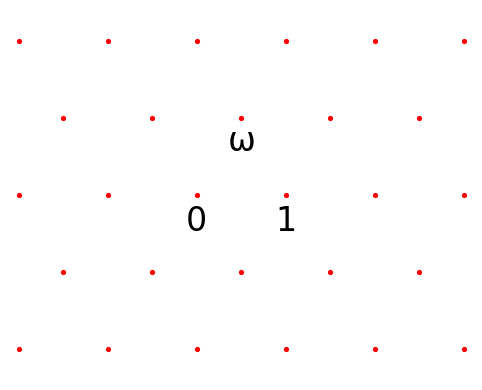
\includegraphics[width=0.3\textwidth]{./plots/lattice.png}
  \end{figure}
\end{beispiel}

Gegeben sei ein Gitter $\Omega$ in $\IC$, wir können dazu eine Funktion
konstruieren. Für $z\in \IC\ssm\Omega$ definieren wir
\begin{equation}
  \label{def:wp}
  \wp_\Omega(z) = \frac{1}{z^2} + \sum_{\omega\in \Omega\ssm\{0\}}
  \left(\frac{1}{(z-\omega)^2} - \frac{1}{\omega^2}\right).
\end{equation}

\begin{bemerkung}
  Die Reihe (\ref{def:wp}) konvergiert absolut für alle
  $z\in\IC\ssm\Omega$.
  Für $\omega\not=0$ und
  $\omega\not=z$ ist der
  Absolutbetrag von 
  \begin{equation*}
    \frac{1}{(z-\omega)^2} - \frac{1}{\omega^2} =
    \frac{\omega^2 - (z-\omega)^2}{(z-\omega)^2\omega^2}
    =\frac{-z^2 + 2z\omega}{(z-\omega)^2\omega^2}
  \end{equation*}
  höchstens $C(z)/|\omega|^3$, wobei $C(z)>0$ von $\omega$ unabhängig
  ist. 
\end{bemerkung}

Ohne Beweis halten wir die folgenden Fakten fest.
Die Abbildung $z\mapsto \wp_\Omega(z)$ ist wohldefiniert und komplex
differenzierbar auf $\IC\ssm\Omega$. Sie ist eine sogenannte meromorphe Funktion
mit einer doppelten Polstelle an jedem Punkt auf $\Omega$. 
Man nennt $\wp_\Omega$ die zu $\Omega$ gehörige \emph{Weierstrass-$\wp$
  Funktion}\index{Weierstrass-$\wp$ Funktion}.

\begin{lemma}
  Sei $\Omega$ eine Gitter in $\IC$ und $\wp_\Omega$ die Funktion
  oben. Für alle $z\in\IC\ssm\Omega$ erfüllt die Ableitung
  \begin{equation}
    \label{eq:wpderiv}
    \wp_\Omega'(z) = -2 \sum_{\omega\in\Omega} \frac{1}{(z-\omega)^3}.
  \end{equation}
  Für alle $z\in\IC\ssm\Omega$ und alle  $\omega\in\Omega$
  gilt $\wp_\Omega(z+\omega) = \wp_\Omega(z)$ und
  $\wp'_\Omega(z+\omega) = \wp'_\Omega(z)$.
\end{lemma}
\begin{proof}
  Die Formel für die Ableitung folgt aus (\ref{def:wp}), man darf
  summandenweise Ableitung, da die Reihe absolut konvergiert. Es gilt
  $\wp'_\Omega(z+\omega) = \wp'_\Omega(z)$ wie im zweiten Teil der
  Aussage, da die Summe (\ref{eq:wpderiv}) invariant unter Translation
  von $z$ wieder in $\Omega$ list. 
  Es folgt damit
  $$
  \wp_\Omega(z+\omega) = \wp_\Omega(z) + c(\omega)
  $$
  wobei $c(\omega)$ nur von $\omega$ aber nicht von $z$ abhängt.
  Wir setzen $z=-\omega/2$ ein und finden
  $\wp_\Omega(\omega/2) = \wp_\Omega(-\omega/2) + c(\omega)$.
  Aber man kann sich aus (\ref{def:wp}) davon überzeugen, dass
  $\wp_\omega(z)=\wp_\omega(-z)$ gilt, d.h. $\wp_\omega$ ist eine
  gerade Funktion. Es folgt $c(\omega)=0$. 
\end{proof}

\begin{bemerkung}
  Sowohl $\wp_\Omega$ wie auch $\wp'_\Omega$ sind \emph{doppelperiodische
    Funktionen}. Deshalb werden die Elemente aus $\Omega$ auch
  Perioden genannt. 
\end{bemerkung}

Ohne Beweis erwähnen wir, dass $\wp_\Omega$ eine wichtige
Differentialgleichung erfüllt. Genauer, es gibt $g_2=g_2(\Omega),g_3=g_3(\Omega)\in\IC$, so
dass
\begin{equation}
  \label{eq:discg2g3}
  g_2^3-27g_3^2 \not=0
\end{equation}
und 
\begin{equation}
  \label{eq:weierstrassdgl}
  {\wp_\Omega'}^2  = 4 \wp_\Omega^3 - g_2\wp_\Omega - g_3.  
\end{equation}


Bis auf den Faktor $4$ liegen die Werte des Paars
$(\wp_\Omega,\wp'_\Omega)$ auf einer elliptischen Kurve. 
Die Bedingung (\ref{eq:discg2g3}) entspricht dabei der Bedingung
(\ref{eq:disccondition}).

Der Faktor $4$ ist harmlos, wir können die gesamten Überlegungen aus
Kapitel~\ref{kap:ek} auf die \emph{modifizierte Weierstrass-Gleichung}
\begin{equation}
  \label{eq:modweierstrass}
  Y^2 = 4X^3-g_2X-g_3 \quad\text{wobei}\quad   g_2^3-27g_3^2 \not=0
\end{equation}
anwenden und ein Gruppengesetz auf $E(\IC)$ definieren.

Wir definieren eine Abbildung
\begin{alignat*}1
  \Psi \colon &\IC\rightarrow E(\IC)
\end{alignat*}
durch
\begin{equation*}
  \Psi(z) = \left\{
    \begin{array}{ll}
      (\wp_\Omega(z),\wp'_\Omega(z)) &: z\not\in\Omega, \\
      \cO &:z\in \Omega.
    \end{array}\right.
\end{equation*}

Wegen der Doppelperiodizität von $\wp_\Omega$ und $\wp'_\Omega$
gilt $\Psi(z+\omega) = \Psi(z)$ für alle $z\in\IC$ und alle
$\omega\in\Omega$.

Weiterhin, und dies ist nicht trivial, ist $\Psi$ ein
Gruppenhomomorphismus, wobei wir $\IC$ als additive Gruppe des Körpers
der komplexen Zahlen verstehen. Schliesslich ist $\Psi$ auch eine
surjektive Abbildung. Aus diesen Überlegungen folgt, dass
\begin{equation*}
  \IC/\Omega \quq E(\IC)\quad\text{vermöge $\Psi$ als Gruppen isomorph sind.}
\end{equation*}

Weiterhin können trägt $E(\IC)$ wegen der Interpretation aus Abschnitt
\ref{sec:projektiv} die Struktur eines topologischen Raums.
Aus
topologischer Sicht sind $\IC/\Omega$ und $E(\IC)$ ununterscheidbar.

\begin{bemerkung}
  Aus topologischer Sicht ist $\IC/\Omega$ nichts anderes als ein
  Torus, vgl. Abbildung~\ref{fig:torus}.
    \begin{figure}
      \centering
      \caption{Ein Torus}
    \label{fig:torus}
    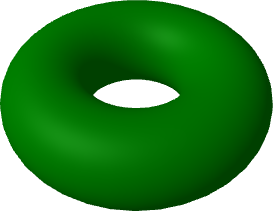
\includegraphics[width=0.3\textwidth]{./plots/torus.png}
  \end{figure}
  Topologisch gesehen sehen alle elliptischen Kurven über $\IC$ gleich
  aus. Aber die elliptische Kurve selber trägt zusätzliche Struktur,
  da sie schlussendlich von einer Weierstrass-Gleichung kommt. Diese
  Struktur ist feiner als die Topologie.
\end{bemerkung}

\begin{bemerkung}
  Sei $\Omega$ ein Gitter in $\IC$ mit Basis $(\omega_1,\omega_2)$ Die
  Halbperioden $\omega_1/2,\omega_2/2,(\omega_1+\omega_2)/2$
  repräsentieren Elemente der Ordnung $2$ in $\IC/\Omega$.
  Wie für die übliche Weierstrass-Gleichung, ohne den Faktor $4$, kann
  man zeigen, dass die Ordinate eines Punktes der Ordnung $2$
  verschwindet.
  Folglich gilt
  \begin{equation*}
    \wp'_\Omega\left(\frac{\omega_1}{2}\right)=
    \wp'_\Omega\left(\frac{\omega_2}{2}\right)=
    \wp'_\Omega\left(\frac{\omega_1+\omega_2}{2}\right)=0. 
  \end{equation*}
  Es folgt, dass
  \begin{equation*}
    \wp_\Omega(z) \text{ eine Nullstelle von }
    4X^3 -g_2(\Omega) X - g_3(\Omega)  \text{ ist für alle }
    z\in \left\{\frac{\omega_1}{2},
      \frac{\omega_2}{2},
      \frac{\omega_1+\omega_2}{2}\right\}.
  \end{equation*}
  Also kann man kubische Gleichungen mit der Hilfe von der
  Weierstrass-$\wp$ Funktion lösen.
\end{bemerkung}

Eine modifizierte Weierstrass-Gleichung (\ref{eq:modweierstrass}) legt
ein Gitter $\Omega$ in $\IC$ fest, für welches
(\ref{eq:weierstrassdgl}) gilt.  Die ``Perioden'' in $\Omega$ lassen
sich durch  Integrale
\begin{equation*}
  \int \frac{dx}{\sqrt{4x^3-g_2 x - g_3}}
\end{equation*}
bestimmen. Das Integral findet auf bestimmten Schleifen  in $\IC$ statt
und der Wert des Integrals hängt auch von der Schleife ab.  Diese
Integrale heissen aus historischen Gründen \emph{elliptischen
  Integrale} und sind verantwortlich für den Begriff ``elliptisch'' in
elliptische Kurve.\footnote{Elliptische Kurven sind keine Ellipsen!}

%%% Local Variables:
%%% TeX-master: "main"
%%% End:



\chapter{Anwendungen}

In diesem Abschnitt untersuchen wir die folgenden
zwei Anwendungen der Theorie
elliptischer Kurven:

\begin{itemize}
\item Der Diffie-Hellman Schlüsselaustausch mit elliptischen Kurven
\item Lenstras (probabilistisches)
  Faktorisierungsverfahren für natürliche Zahlen
\end{itemize}

Für beide Anwendungen arbeiten wir nicht, wie in den ersten
Abschnitten, mit elliptischen Kurven über dem Körper $\IQ,\IR$ oder
$\IC$. Sondern wir werden mit elliptischen Kurven über einem endlichen
Körper oder gar einem endlichen Ring arbeiten. 

\section{Diffie-Hellman Schlüsselaustausch}

Der Diffie-Hellman Schlüsselaustausch liefert eine Lösung für das
folgende Problem.

Zwei Personen, hier $A$ und $B$ genannt, können nur über einem offenen
(und unsicheren!)
Kanal miteinander kommunizieren. Dies könnte z.B. eine
nicht-abhörsichere Telefonleitung sein oder die beiden kommunizieren
über Postkarten. Beide möchten sich auf ein gemeinsames Geheimnis
einigen. In den Anwendungen ist dieses gemeinsame Geheimnis z.B. der
Schlüssel für ein symmetrisches Verschlüsselungsverfahren wie 
AES. Sobald dieser gemeinsame Schlüssel beiden vorliegt, können A
und B  verschlüsselt miteinander kommunizieren. Beim
Bilden des gemeinsamen Schlüssels müssen A und B davon ausgehen, dass
Unbekannte zuhören. Es soll schlussendlich verhindert werden, dass
diese keinen Rückschlüsse auf das Geheimnis machen können.

Der Schlüsselaustausch funktioniert wie folgt.

\bigskip
\textbf{Schritt 1.} A und B legen a priori 
eine grosse Primzahl $p$ und damit einen endlichen Körper $\IF_p$ fest.
Sie einigen sich weiterhin auf eine elliptische Kurve
$$E: Y^2 = X^3+aX+b$$
wobei $a,b\in\IF_p$ und auf einen Punkt $P\in
E(\IF_p)\ssm\{\cO\}$. Die Sicherheit wird gewährleistet, wenn $p$
``gross'' ist und wenn die Ordnung von $P$ als Element der abelschen
Gruppe auch eine grosse  Primzahl.  
\footnote{Der einfachheitshalber arbeiten wir hier
  mit nicht mit langen Weierstrass-Gleichungen. In Anwendungen kommt
  z.B. die Primzahl 
 $p = 2^{255}-19$ und die elliptische Kurve
  $E: Y^2 = X^3+486662X^2+X$ mit langer Weierstrass-Gleichung vor. Der
rationale Punkt $P$ hat die Form $(9,*)$. Er erzeugt eine Untergruppe
von $E(\IF_p)$ dessen Ordnung die Primzahl $\#E(\IF_p)/8$ ist.}
Die gesamte Information $(p,E,P)$ ist an dieser Stelle rein
öffentlich. 
A und B müssen davon ausgehen, dass dritte Zugriff auf
diese Information haben.
Es gibt standardisierte Wahlen für  dieses Tripels in den Implementationen.

\bigskip
\textbf{Schritt 2.} In diesem Schritt wählt A per Zufall eine
natürliche Zahl $a$, die optimalerweise teilerfremd zur Ordnung von
$P$ ist. \emph{Die Zahl $a$ muss geheim bleiben}, nur A kennt sie. A berechnet nun den Punkt
$$
a\cdot P = \underbrace{P+P+P+\cdots + P}_{\text{$a$ mal}}
$$
als Element von $E(\IF_p)$. 

Diese Berechnung lässt sich wie folgt effizient gestalten.
Ist die Entwicklung von $a$ zur Basis $2$ durch $\sum_{i} a_i 2^i$ mit
$a_{i}\in \{0,1\}$ gegeben, so gilt
$$
a\cdot P =\sum_{i : a_i=1} 2^i \cdot P.$$
Also lässt sich $a \cdot P$ rein aus der  Addition $E(\IF_p)\times
E(\IF_p)\rightarrow E(\IF_p)$  und Iterationen der
Verdoppelungsabbildung  $2\colon E(\IF_p)\rightarrow E(\IF_p)$
bestimmen. Die Anzahl Rechenschritte ist in der Grössenordnung $\log
a$. Da $a$ von Grössenordnung $p$ ist, sind das $O(\log p)$
Rechenschritte. 

\bigskip
\textbf{Schritt 3.} B macht das gleiche und wählt eine geheime natürliche Zahl
$b$. Daraufhin berechne $B$ den Punkt $b\cdot P \in E(\IF_p)$.

\bigskip
\textbf{Schritt 4.} Bis an hin wurde noch keine Information zwischen A
und B ausgetauscht (bis auf die Wahl von $(p,E,P)$ die öffentliche
Information ist.)
In Schritt 4 schickt A den Punkt $a\cdot P$ an B. Gleichzeitig schickt
B den Punkt
$b\cdot P$ an A. Dieser Informationsaustausch geschieht auf dem
öffentlichen und unsicheren Kanal. 


\bigskip
\textbf{Schritt 5.} Zu diesem Zeitpunkt besitzt A die Information $a$
und $b\cdot P$ und $B$ besitzt die Information $b$ und $a\cdot P$.

Nun berechnet A den neuen Punkt
\begin{equation*}
  a\cdot (b\cdot P) \in E(\IF_p).
\end{equation*}
Auf der anderen Seite des Kanals berechnet B den Punkt
\begin{equation*}
  b\cdot (a\cdot P) \in E(\IF_p).
\end{equation*}

Nun sind wir am Ziel. Da $E(\IF_p)$ eine Gruppe ist,
gilt
$$
a\cdot (b\cdot P) = (ab)\cdot P = (ba) \cdot P = b\cdot (a\cdot P),$$
diese Gleichung wurde bereits in (\ref{eq:actionofZ}) angesprochen.

Das gemeinsame Geheimnis ist der Punkt $(ab)\cdot P$. Dieses kann als
Grundlage für die Festlegung eines Schlüssel für ein symmetrisches
Verfahren genutzt werden.

\bigskip

Dieses Verfahren ist zur Zeit sicher, da es  keinen  effizienten Weg
gibt, den Wert $a$ (modulo $\mathrm{ord}(P)$)
aus $a\cdot P$ zu rekonstruieren. Diese Problem nennt sich
\emph{diskreter Logarithmus}.

In der Praxis ist $\mathrm{ord}(P)$ von der Grössenordnung $p$ und
damit in Anwendungen ca. $2^{256}$. Einfaches ``Absuchen'' von $a$ ist
nicht praktikabel.

Dennoch ist es nicht ausgeschlossen, dass es einen noch unbekannten
und effizienten Zugang zum diskreten Logarithmus gibt. Dabei bedeutet
``effizient'' ein Algorithmus der mit hoher Wahrscheinlichkeit $a$
produziert und zwar in $O((\log p)^C)$ Rechenschritt für eine Konstante
$C$.

Im Jahr 1994 hat Peter Shor~\cite{shor} einen ``Quantum-Algorithmus'' entwickelt,
welcher den Diffie-Hellman Schlüsselaustausch unsicher macht, sollte
ein hinreichend mächtiger Quantencomputer zur Verfügung stehen.
Kurzum, die zukünftige Bedeutung des Diffie-Hellman
Schlüsselaustausches ist offen.

Eine einfache Implementation des Diffie-Hellman Schlüsselaustausches ist als SageMath Skript
auf der GitHub repository in
\begin{center}
  \href{https://github.com/philipphabegger/ElliptischeKurvenDMK/blob/master/sage/diffie-hellman-schluesselaustausch.ipynb}{\texttt{sage/diffie-hellman-schluesselaustausch.ipynb}}
\end{center}
zu finden.

\section{Lenstras Verfahren}

Gegeben sei eine natürliche zusammengesetzte Zahl $n\ge 2$.
Die Sicherheit des kryptographischen Verfahren RSA beruht auf der (angeblichen)
Schwierigkeit einen Primfaktor von $n$ zu finden.\footnote{Im
  konkreten Fall von RSA ist $n$ ein Produkt $pq$ aus zwei
  verschiedenen Primzahlen
  der Grössenordnung $2^{2048}$.}


Da $n$ zusammengesetzt ist, besitzt $n$ einen Primzahl $p$, so dass
$p\le \sqrt{n}$. Durch simples ausprobieren kann man mit ca. $\sqrt n$
ggT-Operationen $p$ finden. Aber für $n\cong 2^{2048}$ sind das ca.
$2^{1024}> 10^{300}$ Operationen. 

Lenstras Faktorisierungsverfahren ist ein probabilistischer
Algorithmus, um in Laufzeit ca. $e^{\sqrt{2\log n}\sqrt{\log\log n}}$
einen Primfaktor von $n$ zu finden. ``Probabilistisch'' bedeutet, dass
der Algorithmus mit ``grossen Wahrscheinlich'' zum Ziel führt. D.h. es
ist nicht mathematisch gesichert, dass der gesuchte Faktor gefunden
wird. Aber dennoch ist es aus sicherheits-theoretischen Überlegungen
wichtig, solche Algorithmen bei der Wahl eines kryptographischen
Systems zu berücksichtigen.

In der gleichen Arbeit~\cite{shor} hat Shor gezeigt, dass das
Faktorisierungsproblem für einen hinreichen starken Quantencomputer
in polynomialer Zeit (in $\log n$) bewältigbar ist.

Lentsras Faktorisierungsverfahren beruht auf der Theorie
elliptischer Kurven. Nun müssen wir jedoch einen Schritt weiter gehen
als bis an hin. Wir betrachten Weierstrass-Gleichungen mit
Koeffizienten in einem Ring, hier typischerweise $\IZ/n\IZ$. Da
$n$ in der Problemstellung gerade keine Primzahl ist, ist $\IZ/n\IZ$
kein Körper, es ist ein kommutativer Ring mit (nicht-trivialen)
Nullteiler. Wir werden nicht die Theorie elliptischer Kurven über
einem Ring entwickeln,\footnote{Solche Objekte heissen
  \emph{elliptische Schemata} oder \emph{abelsche Schemata}}
sondern  \textit{ad hoc} so rechnen, wie wir das in Abschnitt
\ref{kap:ek} über einem Körper beschrieben haben. Dabei sind einige
Vorkehrungen nötig, um Nullteiler zu berücksichtigen. 
Es sind aber
gerade die Nullteiler von $\IZ/n\IZ$, welche Rückschlüsse auf die
Primfaktoren von $n$ schliessen lassen.

Wir werden die folgende Notation verwenden. Gegeben sei $n\in\IN$. Eine ganze Zahl $a\in\IZ$
 repräsentiert eine Nebenklasse
$$
\overline a = a+n\IZ\in \IZ/n\IZ.
$$
Also verwenden wir $\overline a$ um die Nebenklasse zu beschreiben. 

Gegeben seien $a,b\in\IZ$ und die Gleichung $E : Y^2= X^3+\overline a
X + \overline b$ mit Koeffizienten in $\IZ/n\IZ$. Wir können die
Diskriminante
$$\Delta_E = \overline{-2^4(4a^3+27b^2)}\in\IZ/n\IZ$$ definieren. Aber die Bedingung $\Delta_E\not=0$
reicht in dieser Situation nicht aus, um $E$ als ``elliptische Kurve''
bezeichnen zu dürfen, den $\IZ/n\IZ$ besitzt Nullteiler. Wir brauchen
die stärkere Bedingung $\Delta_E \in (\IZ/n\IZ)^\times$, dabei
bezeichnet $(\IZ/n\IZ)^\times$ die Elemente in $\IZ/n\IZ$ die sich
multiplikativ invertieren lassen.\footnote{Für $n$ eine Primzahl ist $\IZ/n\IZ$
ein Körper und die Bedingung ist mit $\Delta_E\not=0$
gleichbedeutend.}

Die in
Abschnitt~\ref{kap:ek} beschrieben Vorschrift definiert nur eine
partielle Verknüpfung auf 
\begin{equation*}
E(\IZ/n\IZ) =   \{(x,y) \in (\IZ/n\IZ)^2:  y^2 = x^3+\overline a x +
\overline b\}\cup\{\cO\}. 
\end{equation*}
% $Y^2 = X^3+\overline a X +\overline b$ in $(\IZ/n\IZ)^2$ zusammen mit
% $\{\cO\}$. 

Es gilt
\begin{equation}
  \label{eq:ggTDeltaE}
  \Delta_E \in (\IZ/n\IZ)^\times\Longleftrightarrow
  \mathrm{ggT}(-2^4(4a^3+27b^2),n) = 1.
\end{equation}

In der Praxis lässt sich der ggT sehr effizient mittels Teilung
mit Rest berechnen. 
%Diese Aussage ist für unser Anliegen interessant.
Sollte $\Delta_E$
\emph{keine} Einheit sein, dann haben die ``nicht reduzierte''
Diskriminante $-2^4(4a^3+27b^2)$ und $n$ einen gemeinsamen Teiler
$d>1$. Nun gibt es zwei Fälle:

\begin{itemize}
\item \textbf{Fall 1: Es gilt  $d=n$.}  In diesem Fall haben wir leider
  nichts gewonnen
\item \textbf{Fall 2: Es gilt  $d<n$.}
  Dann ist $d$ ein echten Teiler
  von $n$. Um ein Primfaktor von $n$ zu finden, reicht es, einen
  Primfaktor von $d$ zu finden. Da $d\le n/2$ hat sich das Problem durch
  diesen Schritt exponentiell vereinfacht. Ist $n=pq$ das Produkt verschiedener
  Primzahlen $p$ und $q$ (wie in RSA), so gilt sogar $d=p$ oder $d=q$
  und wir sind im Ziel.
\end{itemize}

Nun beschreiben wir eine vereinfachte Version von Lentras Verfahren.
Gegeben sie $n=pq\in\IN$
das Produkt zweier Primzahlen $p\not=q$. 

\bigskip
\textbf{Schritt 1}. Wir wählen zufällig $a,x,y\in \{0,\ldots,n-1\}$.
Diese repräsentieren
$\overline a,\overline
x,\overline y\in\IZ/n\IZ$.
Dann definieren wir
$$
b = y^2 - x^3 - ax\in \IZ.
$$
Das Paar $(\overline x,\overline y)$ ist eine Nullstelle von $Y^2 -
(X^3+\overline a X +\overline b)$.

\bigskip
\textbf{Schritt 2}. Wir berechnen $\Delta = -2^4(4a^3+27b^2)\in\IZ$.
Falls $\mathrm{ggT}(\Delta,n)>1$, d.h. $\overline\Delta$ ist
\emph{keine} Einheit in $\IZ/n\IZ$, so verwenden wir die Überlegung
direkt unterhalb von (\ref{eq:ggTDeltaE}).
Im (unwahrscheinlichen) Fall 1 kehren wir zurück zu Schritt 1 und wählen eine neue Kurve.
Alternativ kann man Fall 1 a priori ausschliessen, wenn man die
Repräsentanten $a,x,y\in \{0,\ldots,n\}$ klein genug in Funktion von
$n$ wählt, um $|\Delta|<n$ zu erzwingen.

Im Fall 2 muss $d=p$ oder $d=q$ gelten. Wir sind fertig, da ein
Primfaktor von $n$ berechnet wurde. Hier ist entscheidend, dass sich
der ggT schnell berechnen lässt.

Also können wir für das weitere Vorgehen annehmen, dass
$\Delta_E\in(\IZ/n\IZ)^\times$. Damit definiert
$E : Y^2 = X^3+\overline a X + \overline b$ eine (verallgemeinerte) elliptische Kurve
mit Koeffizienten in $\IZ/n\IZ$.

\bigskip
\textbf{Schritt 3}. Wir betrachten das Paar $(\overline x,\overline y)$
als Punkt $P$ in $E(\IZ/n\IZ)$. 
Die in Abschnitt~\ref{kap:ek}, Abschnitt \ref{sec:verknuepfung},
beschriebene Verknüpfung kann man
ad hoc auf die  
Punkte in  $E(\IZ/n\IZ)$ anzuwenden.
Unser Ziel ist es, ein Vielfaches $B \cdot P$ zu berechnen, dabei ist
$B=k!\in\IN$ eine natürliche Zahl. Konkret werden wir $2\cdot P,
6\cdot P, 24\cdot P$  bis zu $B \cdot P$ ausrechnen. 

Um das effizient zu gestalten, entwickeln wir $k$, wie beim
Diffie-Hellman Schlüsselaustausch, zur Basis $2$. D.h. wir schreiben
$k=\sum_{i} k_i 2^i$ mit
$k_{i}\in \{0,1\}$. Wir möchten 
$$
\sum_{i : k_i=1} 2^i \cdot Q
$$
für $Q\in E(\IZ/n\IZ)$ bestimmen.

Insgesamt müssen wir auf $E(\IZ/n\IZ)$   zwei Punkte addieren können.
Da aber $\IZ/n\IZ$ kein Körper ist, darf nicht durch ein Element
ungleich Null dividiert werden. Es gibt  Nullteiler. 
Z.B. im Unterfall 1a wird bei der Konstruktion der Steigung $m$ durch
die Differenz $x_1-x_2$. Oder im Unterfall 2a, bei der Verdoppelung,
wird durch $2y$ geteilt.

Teilen ist jedoch nur erlaubt, wenn das entsprechende Element in
$(\IZ/n\IZ)^\times$ liegt. D.h. bei jeder Teilung müssen wir
überprüfen, dass der ggT eines Repräsentanten in $\IZ$, von $x_1-x_2$ oder $2y$,
zu $n$ gleich $1$ ist. Ist der ggT gleich $1$, so dürfen wir teilen
und die Berechnung durchführen.
Ist der ggT jedoch $>1$ so sind wir wieder in einer
Fallunterscheidungen wie unterhalb von (\ref{eq:ggTDeltaE}).

Sollte $d=n$ gelten, so haben wir ``Pech''. Wir müssen das Verfahren wieder
bei Schritt 1 mit einer neuen Wahl von $\overline a,\overline
x,\overline y$ starten. Es scheint schwierig, diesen unglücklichen
Ausgang a priori auszuschliessen. Deshalb ist dieser Algorithmus
``probabilistisch''.

Gilt jedoch $1<d<n$, so muss (da $n=pq$) $d=p$ oder $d=q$ gelten. In diesem
Fall sind wir fertig, da ein Primfaktor gefunden wurde.

\bigskip

Die genaue Wahl von $B$ spielt für die Analyse des Algorithmus eine
wichtig Rolle auf die wir hier nicht eingehen werden. Anstatt einer
Fakultät, stellt sich als vorteilhaft heraus, für $B$ ein Produkt von
vielen ``kleinen'' Primzahlen zu wählen.

Eine einfache Implementation dieses Verfahrens ist als SageMath Skript
auf der GitHub repository in
\begin{center}
    \href{https://github.com/philipphabegger/ElliptischeKurvenDMK/blob/master/sage/primfaktorisierung_lenstra.ipynb}{\texttt{sage/primfaktorisierung\_lenstra.ipynb}}
\end{center}
zu finden. Hier wurde $B=10!$ festgelegt.





%%% local Variables:
%%% TeX-master: "main"
%%% End:



\appendix
\chapter{Komplexe Multiplikation}

Eines der faszinierendsten Aspekte der Theorie elliptischer Kurven ist
die Möglichkeit komplexer Multiplikation. Diese soll nur an einigen
Beispielen veranschaulicht werden.

Wir beginnen mit einer Weierstrass-Gleichung $E : Y^2=X^3+aX+b$ mit
$a,b$ in einem beliebigen Körper $K$. Wie um (\ref{eq:amultP}) beschrieben,
können wir Punkt $P\in E(K)$ mit ganzen Zahlen multiplizieren, z.B.
$2P = P+P$ und $3P = P+P+P$ etc. Dies ist  in jeder Gruppe möglich.

\begin{beispiel}
  Wir betrachten die elliptische Kurve die durch  $E: Y^2 = X^3+X$
  definiert ist. Der Grundkörper $K$ sei nun $\IC$.
  Sei $(x,y)\in\IC^2$ eine Nullstelle von $Y^2 = X^3+X$. Dann gilt
  \begin{equation*}
    (\sqrt{-1} y)^2 = -y^2 = -(x^3+x) = (-x)^3+(-x). 
  \end{equation*}
  Also ist $(-x,\sqrt{-1}y)$ wieder eine Nullstelle der
  Weierstrass-Gleichung. 
  Für jeden Punkt $P\in E(\IC)$ definiert man
  \begin{equation*}
    I(P) = \left\{
      \begin{array}{ll}
        (-x, \sqrt{-1}y)         &: P = (x,y) \\
        \cO &: P = \cO.
      \end{array}\right.
  \end{equation*}
  Damit erhalten wir eine Selbstabbildung $I\colon E(\IC)\rightarrow
  E(\IC)$.

  Verkettet man $I$ mit sich selbst, so erhält man 
  \begin{equation*}
    I(I(P)) = (x,-y)
  \end{equation*}
  falls $P\not=\cO$. Also ist $I\circ I$ die Inversionsabbildung
  $-\colon E(\IC)\rightarrow E(\IC)$.

  In geeigneter Notation gilt $I^2 = I\circ I = -1$. 

  Man kann nun überprüfen, z.B. von Hand, dass $I$ mit dem
  Gruppengesetz kompatibel ist. D.h. es gilt
  \begin{equation*}
    I(P+Q) = I(P)+I(Q) \quad\text{für alle}\quad P,Q\in E(\IC). 
  \end{equation*}

  Schliesslich kann man weiter und für $\alpha,\beta\in\IZ$ eine
  weiter Selbstabbildung von $E(\IC)$ gemäss
  \begin{equation*}
    (\alpha + I \beta)(P) = (\alpha \cdot P) + (\beta \cdot I(P))
  \end{equation*}
  definieren. 

  Wie identifizieren die Menge $\{\alpha + I\beta :
  \alpha,\beta\in\IZ\}$ der eben definierten Selbstabbildung mit den
  Gaussschen Zahlen
  \begin{equation*}
    \IZ[\sqrt{-1}] = \{\alpha + \sqrt{-1}\beta : \alpha,\beta\in\IZ\}.
  \end{equation*}

  Wir erhalten eine Verknüpfung
  \begin{equation*}
    \IZ[\sqrt{-1}]\times E(\IC)\rightarrow E(\IC)
  \end{equation*}
  welche es uns erlaubt, Punkte in $E(\IC)$ mit Gausssche Zahlen zu
  multiplizieren. Für festes $\gamma\in\IZ[\sqrt{-1}]$ ist der
  Ausdruck $\gamma\cdot P$ ein komplizierter Bruch von Polynomen in
  den Koordinaten von $P$.

  Nicht jede elliptische Kurve erlaubt komplexe Multiplikation. In der
  Tat gibt es (in einem geeigneten Sinn) nur eine elliptische Kurve,
  die komplexe Multiplikation mit $\IZ[\sqrt{-1}]$ wie oben erlaubt.
\end{beispiel}

\begin{aufgabe}
  Überprüfen Sie mit der Definition, dass in der Notation des
  Beispiels oben $I(P+Q) = I(P)+I(Q)$ für alle $P,Q\in E(\IC)$ gilt.
\end{aufgabe}

Es gibt auch eine elliptische Kurven, die ``komplexe Multiplikation'' mit
dem Ring der Eisenstein Zahl
\begin{equation*}
  \left\{\alpha +\beta e^{2\pi\sqrt{-1}/6} : \alpha,\beta\in\IZ\right\}
\end{equation*}
hat. Im Allgemeinen taucht jede ``quadratische Ordnung'', darunter
z.B. auch
\begin{equation*}
  \left\{\alpha +\beta \frac{1+\sqrt{-163}}{2} : \alpha,\beta\in\IZ\right\}
\end{equation*}

Die Theorie der ``komplexen Multiplikation'' von elliptischen Kurven und deren
Verallgemeinerung begann im 19ten Jahrhundert und spielt auch noch
heute in der Grundlagenforschung eine zentrale Rolle~\cite{quanta:ao}.

Komplexe Multiplikation liefert auch eine überzeugende Erklärung,
wieso  
\begin{equation*}
  e^{\sqrt{163}\pi} = 262537412640768743,9999999999992500725971\ldots
\end{equation*}
fast die ganze Zahl  $640320^3 + 744$ ist.

%%% Local Variables:
%%% TeX-master: "main"
%%% End:


\bibliographystyle{alpha}
\bibliography{literature}

%\vfill\hfill
\printindex



\end{document}